\documentclass[ignorenonframetext,]{beamer}
\setbeamertemplate{caption}[numbered]
\setbeamertemplate{caption label separator}{: }
\setbeamercolor{caption name}{fg=normal text.fg}
\beamertemplatenavigationsymbolsempty
\usepackage{lmodern}
\usepackage{amssymb,amsmath}
\usepackage{ifxetex,ifluatex}
\usepackage{fixltx2e} % provides \textsubscript
\ifnum 0\ifxetex 1\fi\ifluatex 1\fi=0 % if pdftex
\usepackage[T1]{fontenc}
\usepackage[utf8]{inputenc}
\else % if luatex or xelatex
\ifxetex
\usepackage{mathspec}
\else
\usepackage{fontspec}
\fi
\defaultfontfeatures{Ligatures=TeX,Scale=MatchLowercase}
\fi
\usetheme{Dresden}
\usecolortheme{seahorse}
% use upquote if available, for straight quotes in verbatim environments
\IfFileExists{upquote.sty}{\usepackage{upquote}}{}
% use microtype if available
\IfFileExists{microtype.sty}{%
\usepackage{microtype}
\UseMicrotypeSet[protrusion]{basicmath} % disable protrusion for tt fonts
}{}
\newif\ifbibliography
\usepackage{graphicx,grffile}
\makeatletter
\def\maxwidth{\ifdim\Gin@nat@width>\linewidth\linewidth\else\Gin@nat@width\fi}
\def\maxheight{\ifdim\Gin@nat@height>\textheight0.8\textheight\else\Gin@nat@height\fi}
\makeatother
% Scale images if necessary, so that they will not overflow the page
% margins by default, and it is still possible to overwrite the defaults
% using explicit options in \includegraphics[width, height, ...]{}
\setkeys{Gin}{width=\maxwidth,height=\maxheight,keepaspectratio}

% Prevent slide breaks in the middle of a paragraph:
\widowpenalties 1 10000
\raggedbottom

\AtBeginPart{
\let\insertpartnumber\relax
\let\partname\relax
\frame{\partpage}
}
\AtBeginSection{
\ifbibliography
\else
\let\insertsectionnumber\relax
\let\sectionname\relax
\frame{\sectionpage}
\fi
}
\AtBeginSubsection{
\let\insertsubsectionnumber\relax
\let\subsectionname\relax
\frame{\subsectionpage}
}

\setlength{\parindent}{0pt}
\setlength{\parskip}{6pt plus 2pt minus 1pt}
\setlength{\emergencystretch}{3em}  % prevent overfull lines
\providecommand{\tightlist}{%
\setlength{\itemsep}{0pt}\setlength{\parskip}{0pt}}
\setcounter{secnumdepth}{0}

\title{Probability calibration methodologies with local expert ensembles}
\subtitle{CPT Nick Normandin}
\date{}

\begin{document}
\frame{\titlepage}

\section{Introduction}\label{introduction}

\begin{frame}{What should you know about this brief?}

\begin{itemize}[<+->]
\tightlist
\item
  \textbf{Please ask questions as I go}
\item
  I've assumed some audience proficiency in modern machine learning
  techniques, but I will alternatively try to provide a heuristic
  understanding of the concepts presented
\item
  Full accompanying R code is available
\item
  This work was funded by the Omar N. Bradley Officer Research
  Fellowship in Mathematics
\end{itemize}

\end{frame}

\begin{frame}{What is \texttt{local\ expert}?}

I created a new kind of ensemble forecasting method that I've called
local expert regression. It involves the decomposition of a supervised
learning task with a continuous target variable (\emph{regression}) into
a series of of many \(\{0, 1\}\) mappings corresponding to separate
\emph{binary probabilistic classification} tasks that produce estimates
on the \([0, 1]\) interval.

\begin{block}{Why is this useful ?!}

Because you can aggregate the ensemble predictions to form a completely
unique \emph{probability distribution function} for each prediction. You
can understand \textbf{risk} not just in terms of a model, but in terms
of each individual forecast.

\end{block}

\begin{block}{\ldots{}see
\textbf{\href{https://github.com/nnormandin/localexpeRt}{github.com/nnormandin/localexpeRt}}}

\end{block}

\end{frame}

\begin{frame}{What problem am I solving?}

\begin{columns}
\begin{column}{0.48\textwidth}

Most classification methods produce scores for class membership which are interpereted as measures of class affiliation probability. This is the foundation of local expert regression. However, these `probabilities' are not usually \textbf{well-calibrated}. 

\end{column}


\begin{column}{0.48\textwidth}
\begin{block}{Definition:}

For a model $f$ and score $s_i$ to be well-calibrated for class $c_i$, the empirical probability of a correct classification $P(c_i | f( c_i | x_i)=s_i)$ must converge to $f(c_i | x_i) = s_i$.

\end{block}
\begin{block}{Example:}

When $s_i = 0.9$, the probability of a correct classification should converge to $P(c_i | s_i = 0.9) = 0.9$. Otherwise, this isn't \textit{really} a `probability.'

\end{block}
\end{column}
\end{columns}

\end{frame}

\begin{frame}{How do I propose to solve it?}

\begin{block}{If probabilities aren't properly calibrated, the PDFs
interpolated from them won't be reliable. How can we deal with this?}

\begin{enumerate}
\def\labelenumi{\arabic{enumi}.}
\tightlist
\item
  Change the loss function

  \begin{itemize}
  \tightlist
  \item
    \(n^{-1}\sum_{i=1}^{n}-y_i\log(p_i)-(1-y_i)\log(1-p_i)\)
  \end{itemize}
\item
  Calibrate probabilities

  \begin{itemize}
  \tightlist
  \item
    isotonic regression, sigmoid transforms?
  \end{itemize}
\end{enumerate}

\end{block}

\end{frame}

\section{Local expert}\label{local-expert}

\begin{frame}{How is local expert different from normal regression?}

\begin{figure}[htbp]
\centering
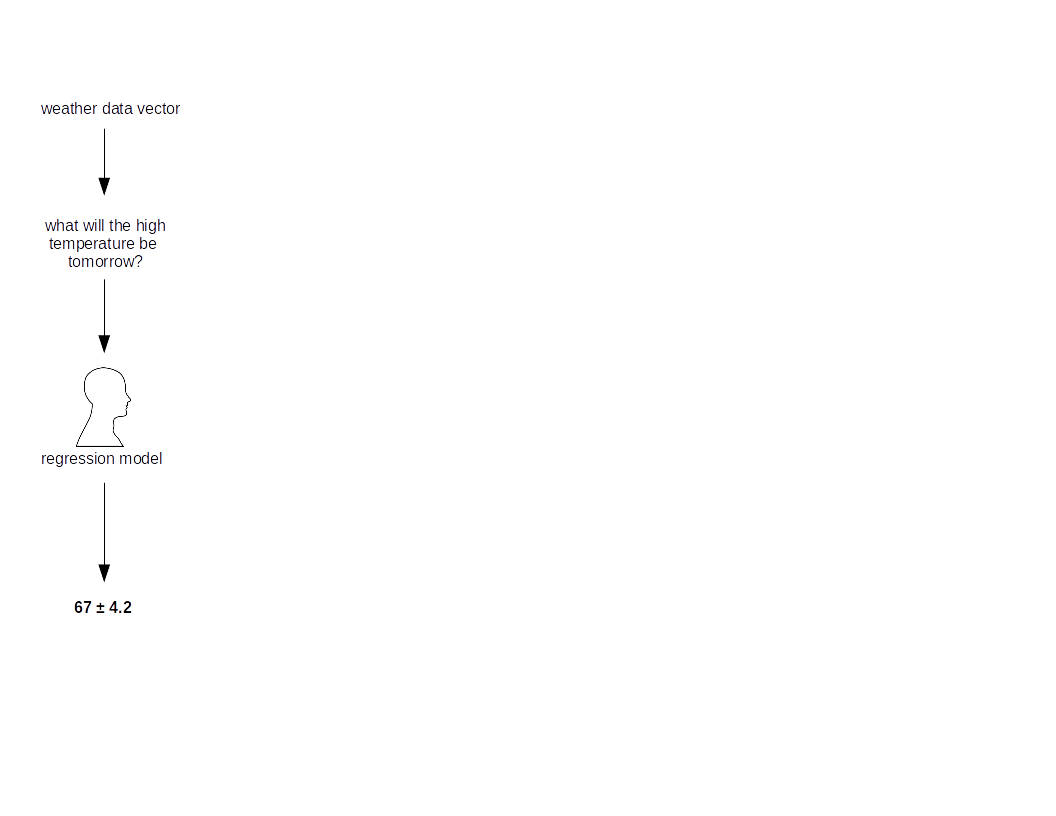
\includegraphics{~/R/projects/MORS_2017/figure1/first.png}
\caption{image}
\end{figure}

\end{frame}

\begin{frame}{How is local expert different from normal regression?}

\begin{figure}[htbp]
\centering
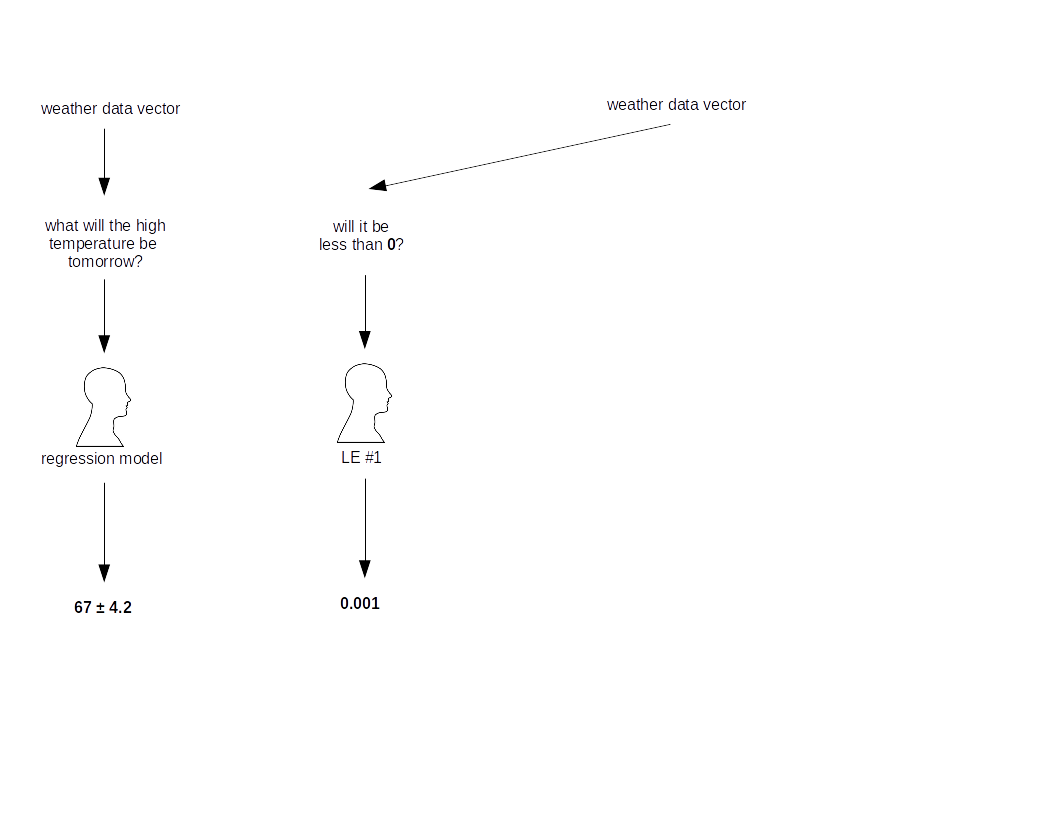
\includegraphics{~/R/projects/MORS_2017/figure1/second.png}
\caption{image}
\end{figure}

\end{frame}

\begin{frame}{How is local expert different from normal regression?}

\begin{figure}[htbp]
\centering
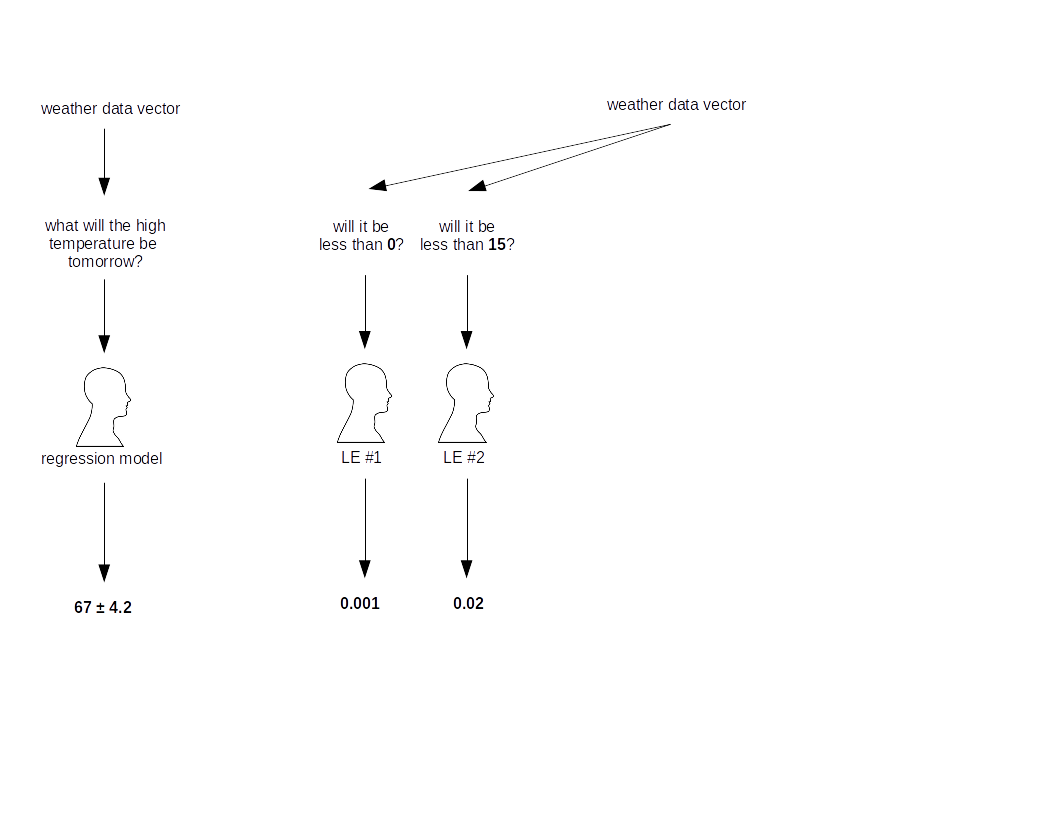
\includegraphics{~/R/projects/MORS_2017/figure1/third.png}
\caption{image}
\end{figure}

\end{frame}

\begin{frame}{How is local expert different from normal regression?}

\begin{figure}[htbp]
\centering
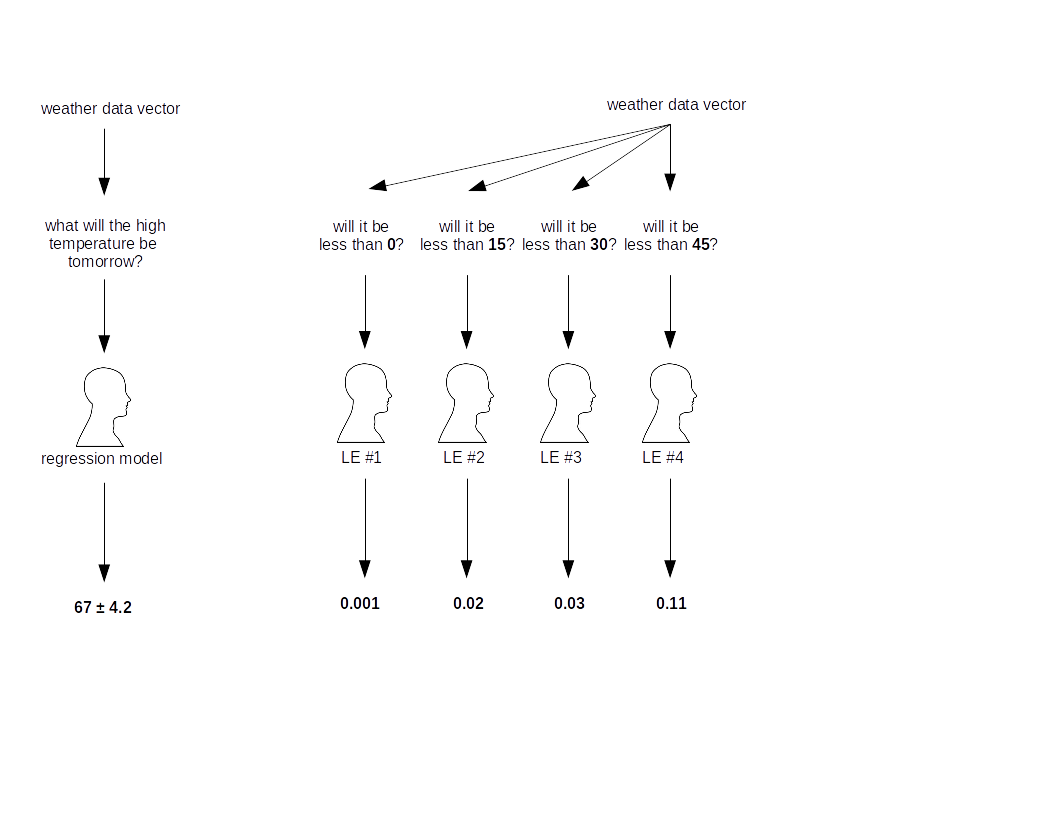
\includegraphics{~/R/projects/MORS_2017/figure1/fourth.png}
\caption{image}
\end{figure}

\end{frame}

\begin{frame}{How is local expert different from normal regression?}

\begin{figure}[htbp]
\centering
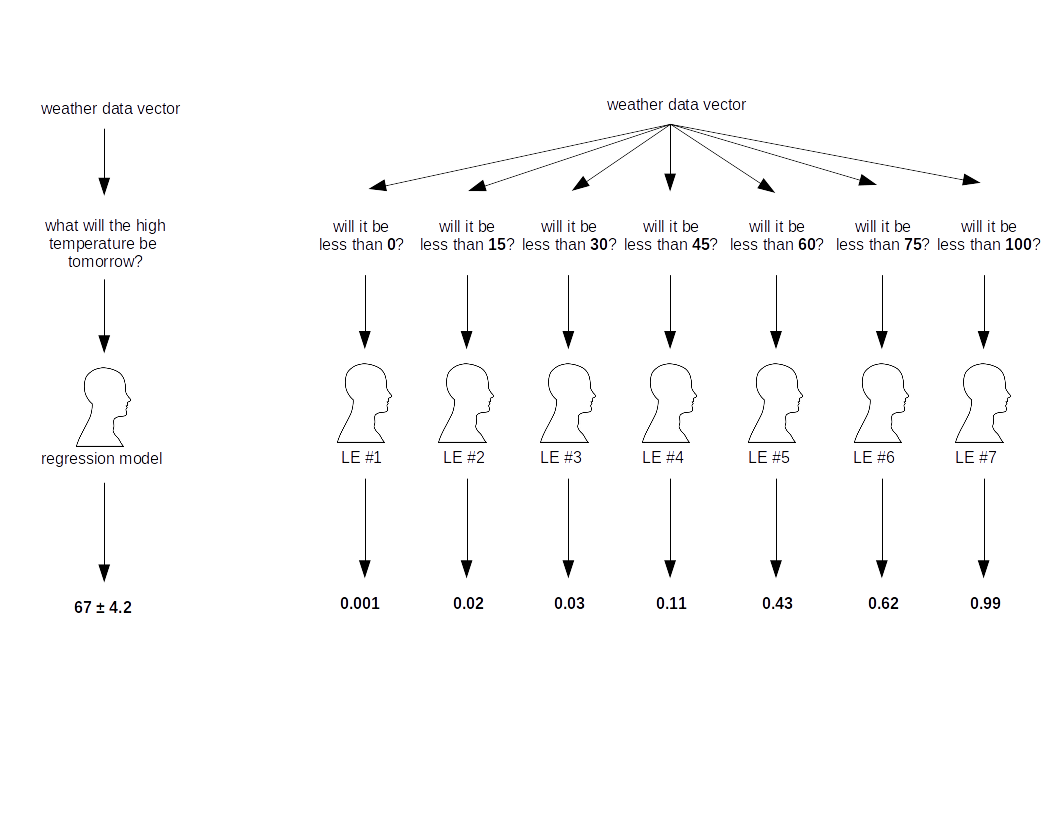
\includegraphics{~/R/projects/MORS_2017/figure1/last.png}
\caption{image}
\end{figure}

\end{frame}

\begin{frame}{How is local expert different from normal regression?}

\end{frame}

\section{Probability calibration}\label{probability-calibration}

\begin{frame}{Why are some model scores poorly calibrated?}

\begin{columns}[t]
\begin{column}{0.48\textwidth}

\begin{block}{$s_i$ dense around 0.5}
\begin{itemize}
\item Maximal margin hyperplanes push scores away from extremes of distribution
\item Common in support vector machines, boosted learners
\end{itemize}
\end{block}

\end{column}


\begin{column}{0.48\textwidth}

\begin{block}{$s_i$ dense around 0, 1}
\begin{itemize}
\item Model assumptions make class probabilites unrealistically confident
\item Naive Bayes!
\end{itemize}
\end{block}
\end{column}
\end{columns}

\end{frame}

\begin{frame}{How can we visualize calibration?}

Cross-validated class probabilities from a naive bayes model trained on
the Pima Indian Diabetes data

\footnotesize
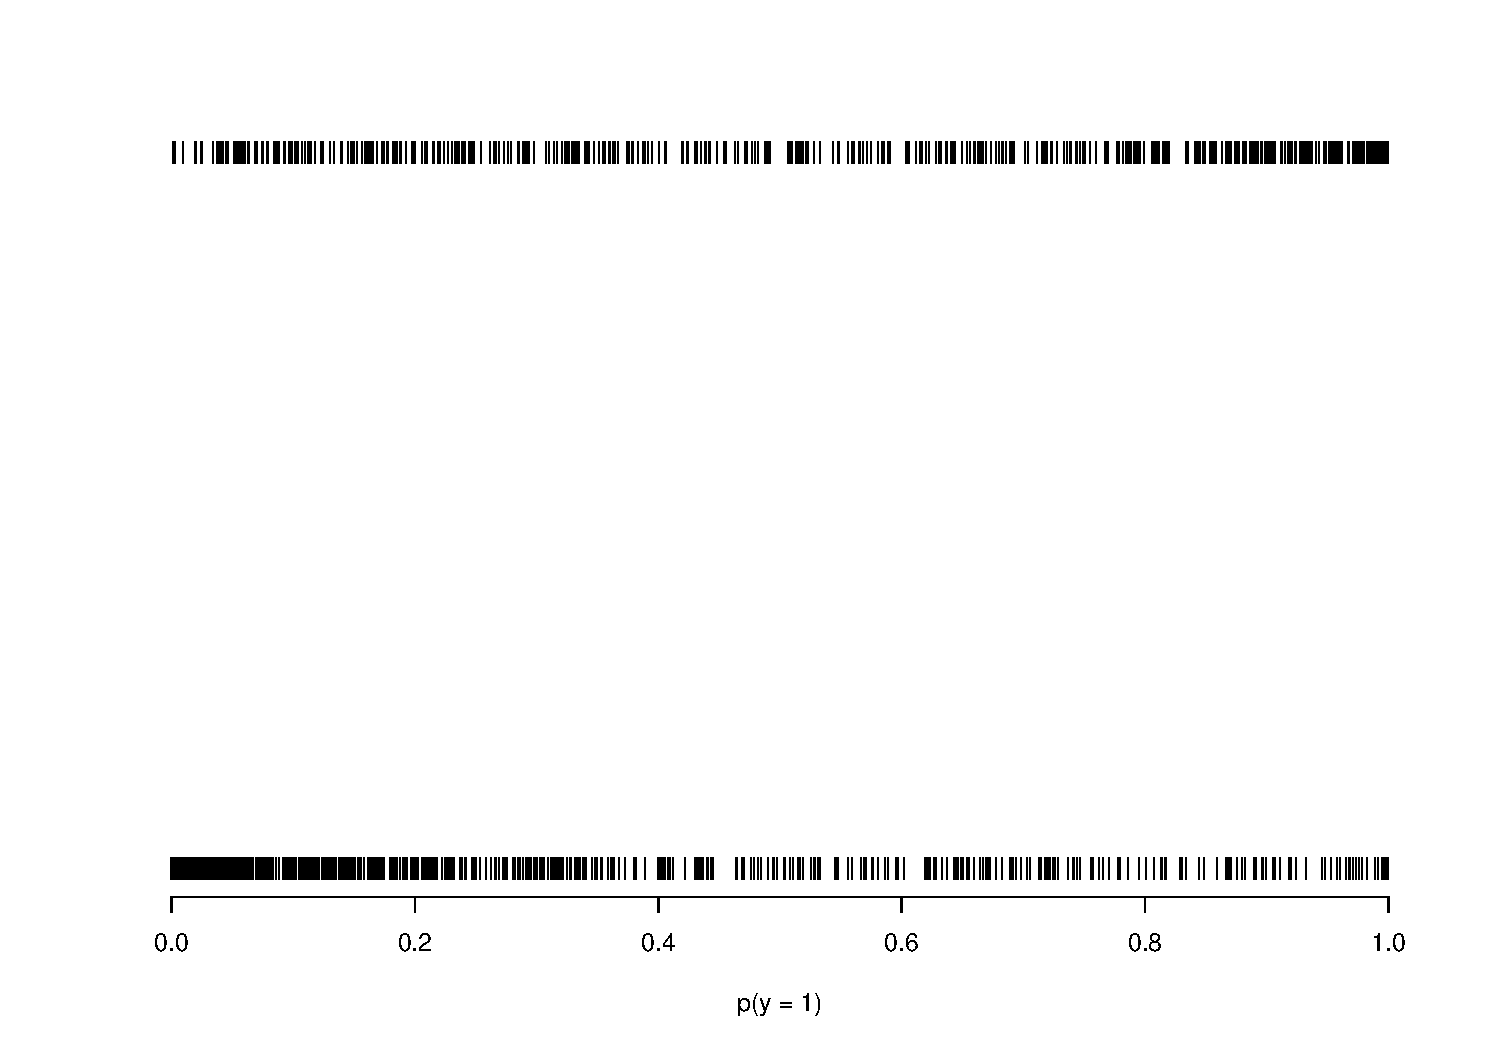
\includegraphics{presentation_files/figure-beamer/unnamed-chunk-1-1.pdf}

\end{frame}

\begin{frame}{How can we visualize calibration?}

Reliability plot: \textbf{(1)} Bin predictions by \(s_i\) (x-axis),
\textbf{(2)} calculate \(p(c_i)\) by bin (y-axis)

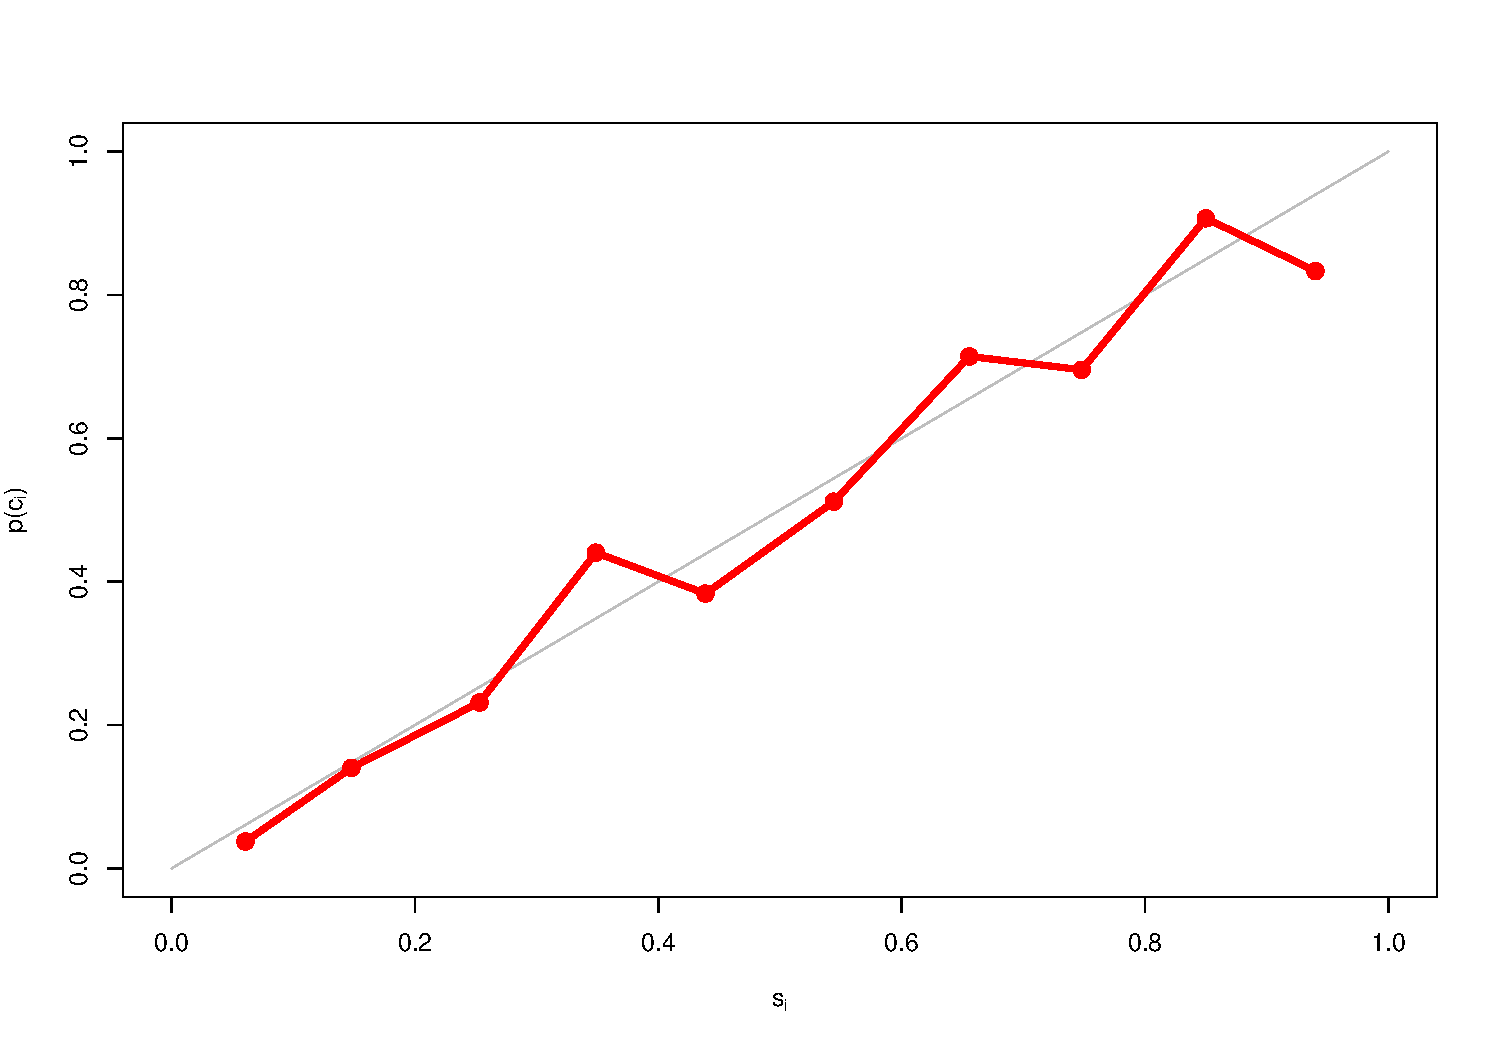
\includegraphics{presentation_files/figure-beamer/unnamed-chunk-2-1.pdf}

\end{frame}

\begin{frame}{Method 1: Isotonic Regression}

A strictly-nondecreasing piecewise linear function \(m\), where
\(y_i = m(s_i) + \epsilon\) fit such that
\(\hat{m} = {argmin}_z \sum_i{y_i-z(s_i) ^2}\).

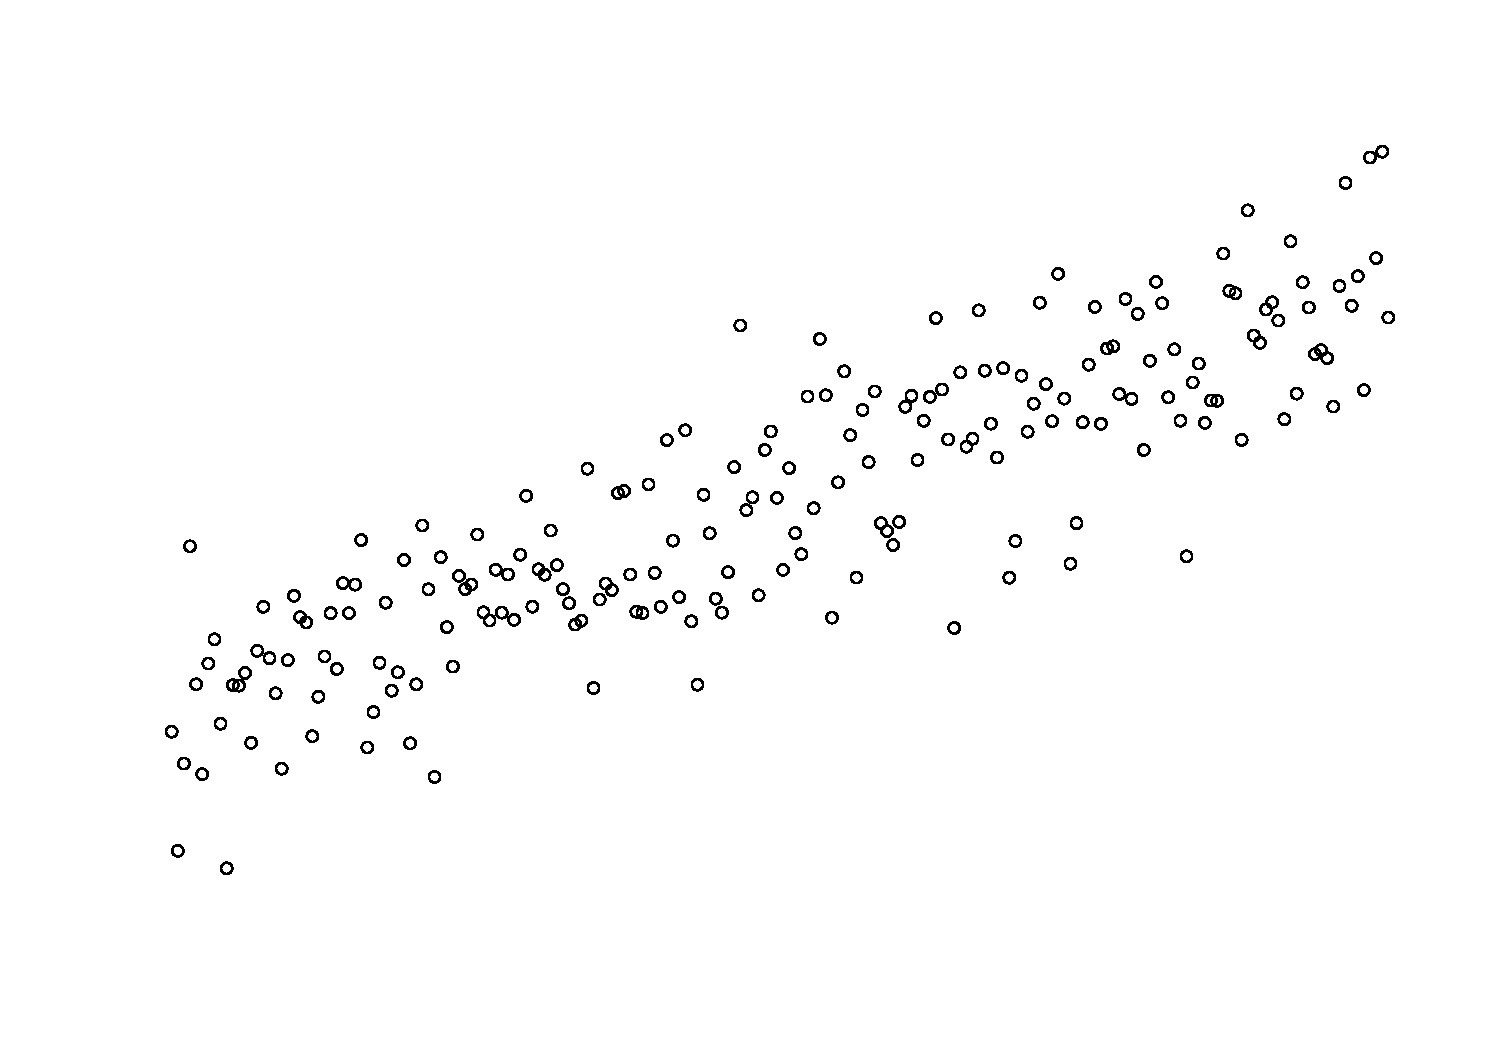
\includegraphics{presentation_files/figure-beamer/unnamed-chunk-4-1.pdf}

\end{frame}

\begin{frame}{Method 1: Isotonic Regression}

A strictly-nondecreasing piecewise linear function \(m\), where
\(y_i = m(s_i) + \epsilon\) fit such that
\(\hat{m} = {argmin}_z \sum_i{y_i-z(s_i) ^2}\).

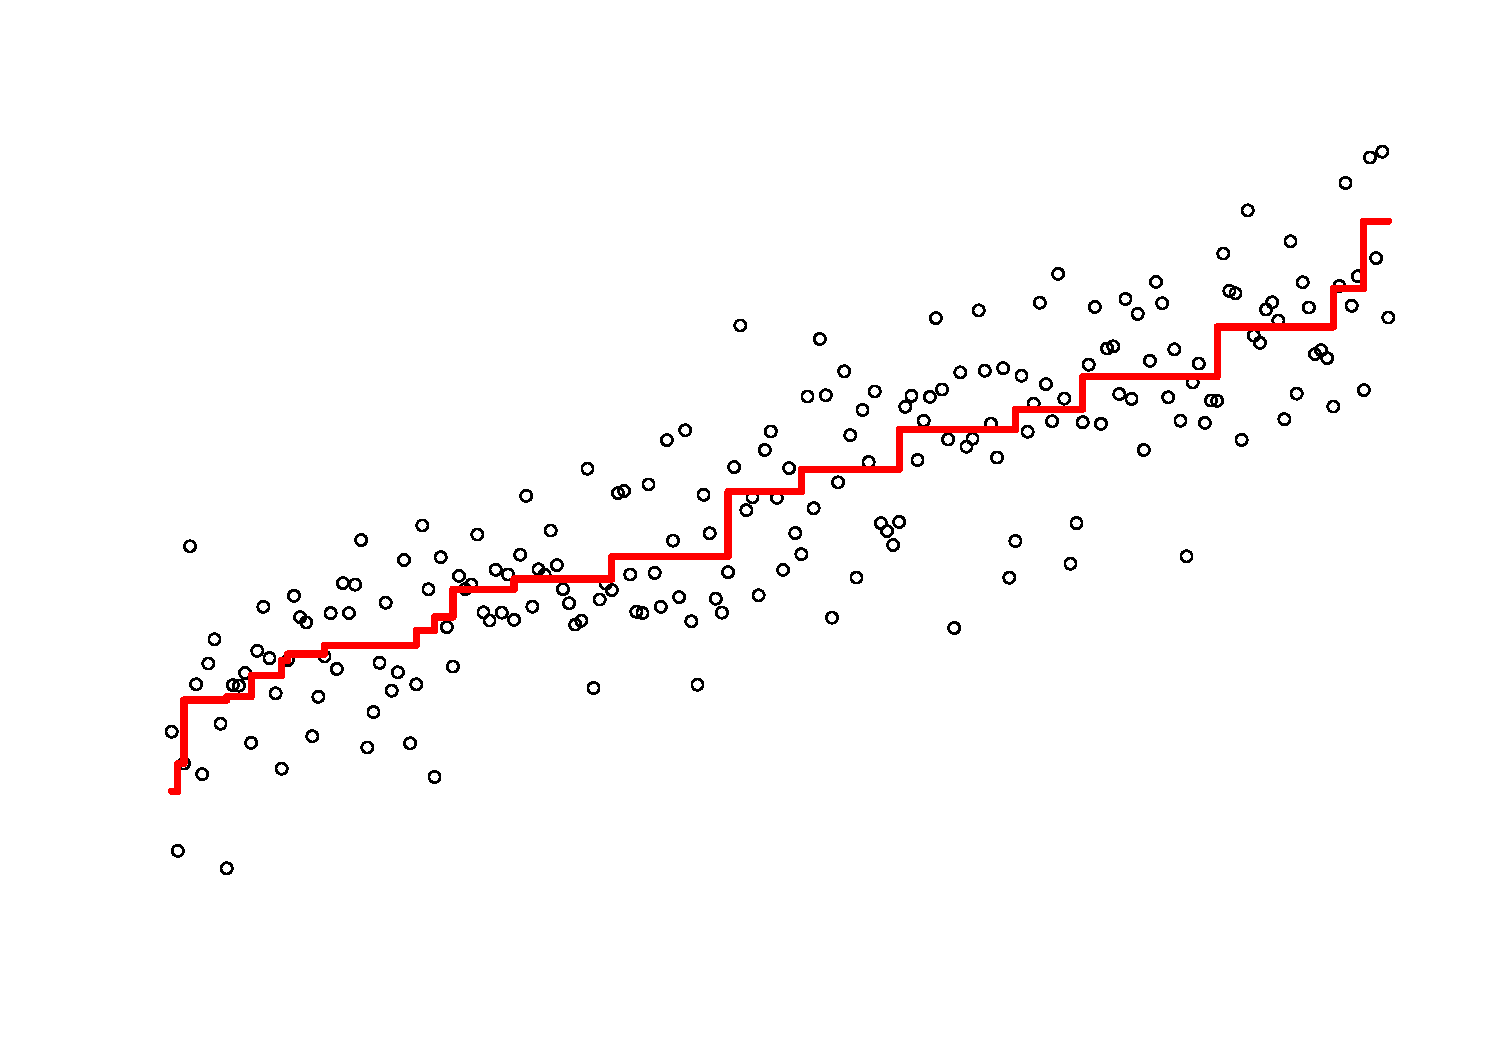
\includegraphics{presentation_files/figure-beamer/unnamed-chunk-5-1.pdf}

\end{frame}

\begin{frame}{Method 2: Platt Scaling}

\end{frame}

\section{Case study}\label{case-study}

\section{Results}\label{results}

\section{Conclusion}\label{conclusion}

\begin{frame}{What have I demonstrated?}

\end{frame}

\begin{frame}{Which topics require more research?}

\begin{enumerate}
\def\labelenumi{\arabic{enumi}.}
\tightlist
\item
  Compensation for class imbalance (SMOTE?)
\item
  Kappa-based optimization methods
\item
  High-level parallelization
\end{enumerate}

\end{frame}

\section{Questions}\label{questions}

\end{document}
